% F3: CE1 -- density 1 that no placement can pack
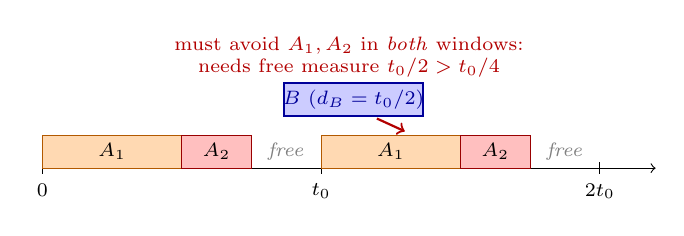
\begin{tikzpicture}[xscale=1.18, yscale=0.6, font=\scriptsize]
  % two base windows [0,t0), [t0,2t0)
  \draw[->] (0,0) -- (6.6,0);
  \foreach \x/\l in {0/0, 3/{t_0}, 6/{2t_0}} {
    \draw (\x,-0.12) -- (\x,0.12);
    \node[below] at (\x,-0.12) {$\l$};
  }
  % A1 (d = t0/2) and A2 (d = t0/4) repeat in EVERY window
  \foreach \o in {0, 3} {
    \fill[orange!30] (\o,0) rectangle (\o+1.5,0.7);
    \draw[orange!70!black] (\o,0) rectangle (\o+1.5,0.7);
    \fill[red!25] (\o+1.5,0) rectangle (\o+2.25,0.7);
    \draw[red!60!black] (\o+1.5,0) rectangle (\o+2.25,0.7);
  }
  \node at (0.75,0.35) {$A_1$};
  \node at (1.875,0.35) {$A_2$};
  \node at (3.75,0.35) {$A_1$};
  \node at (4.875,0.35) {$A_2$};
  % free gaps
  \foreach \o in {0, 3} {
    \node[gray] at (\o+2.625,0.35) {\emph{free}};
  }
  % B's needed contiguous t0/2 interval -- shown failing
  \fill[blue!20] (2.6,1.1) rectangle (4.1,1.8);
  \draw[blue!60!black, thick] (2.6,1.1) rectangle (4.1,1.8);
  \node[blue!60!black] at (3.35,1.45) {$B$ ($d_B = t_0/2$)};
  \draw[->, thick, red!70!black] (3.6,1.05) -- (3.9,0.78);
  \node[red!70!black, align=center] at (3.3,2.35)
    {must avoid $A_1, A_2$ in \emph{both} windows:\\
     needs free measure $t_0/2 > t_0/4$};
\end{tikzpicture}
